\documentclass{article}
\usepackage[shortlabels]{enumitem}
\usepackage[a4paper, total={6in, 8in}]{geometry}
\usepackage{hyperref}
\usepackage{graphicx}
\usepackage{caption}
\title{Work Product}
\author{Mukund Balaji Srinivas\\\textit{mukundbalaji.srinivas@anu.edu.au}}

\begin{document}

\maketitle

\section*{Linkedin Educational Videos}
\begin{itemize}
    \item  (Figure \ref{fig:Linkedin Content }).
    \item (Figure \ref{fig:Linkedin Content-2}).
\end{itemize}


\section*{GradResidence}
\begin{itemize}
    \item Co-founded \href{https://gradresidence.com/}{GradResidence} (Figure \ref{fig:gradResidence}).
    \item Additionally, GradResidence plans to roll out iOS and \href{https://github.com/gradresidence/android}{Android}(Figure \ref{fig:gradResidenceAndroid}).
\end{itemize}

\section*{PMI Canberra}
\begin{itemize}
    \item Contributing to website development projects (Figure \ref{fig:PMI Canberra})
\end{itemize}

\section*{Software Construction}
\begin{itemize}
    \item Participated in the Software Construction (COMP6442) \href{https://gitlab.cecs.anu.edu.au/u7544253/ga-23s1-comp2100-6442} {Project} (Figure \ref{fig:Software Construction})
\end{itemize}

\section*{RattleNG}
\begin{itemize}
    \item Contributed to the development of \href{https://github.com/gjwgit/rattleng}{RattleNG} (Figure \ref{fig:RattleNG})
\end{itemize}


\section*{Appendix}
The Job Posting for \href{https://www.hays.com.au/job-detail/gis-database-engineer-nsw---sydney-cbd_2891906?q=Gis%20Data%20Engineer&location=&applyId=JOB_5120563&jobSource=HaysGCJ&isSponsored=N&specialismId=&subSpecialismId=&jobName=projects%2Fmineral-balm-174308%2Ftenants%2Fab5d683d-f9a5-4b85-bfe0-eb74881e24cf%2Fjobs%2F128663770535731910&lang=en}{GIS Database Engineer} Posted at Hays (Figure \ref{fig:Job with hays}).

\begin{figure}[ht!]
    \centering
    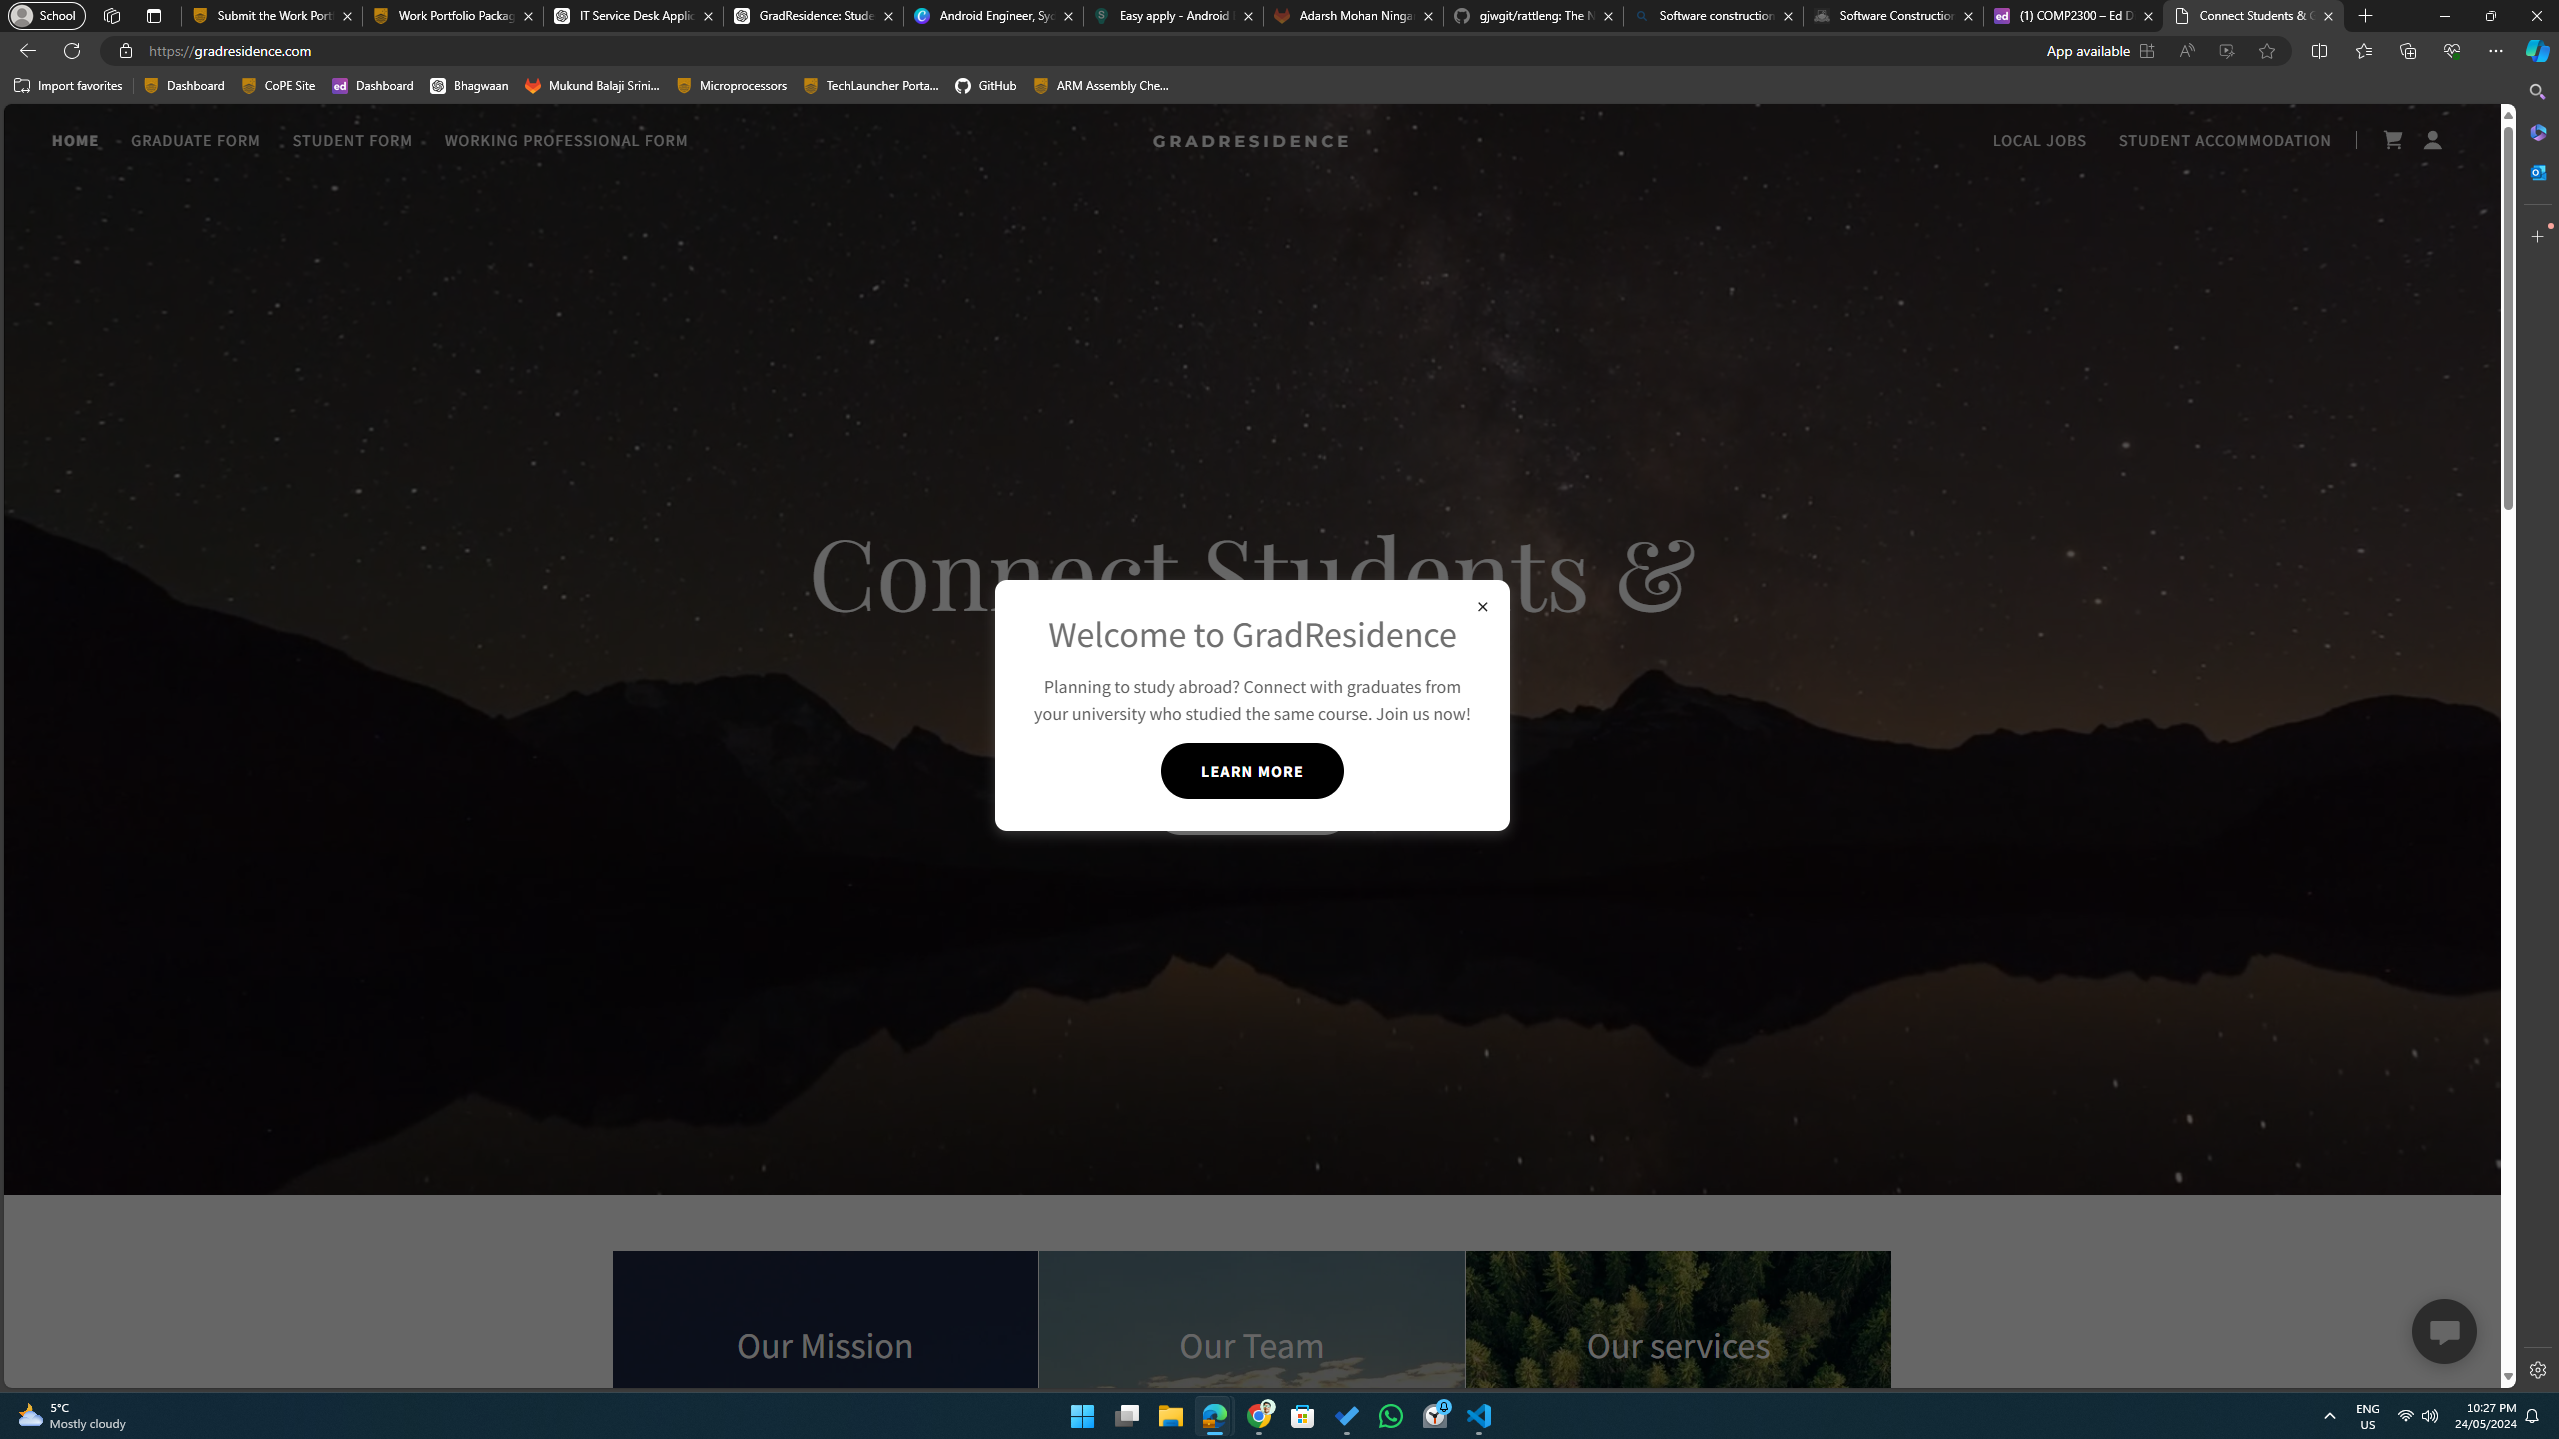
\includegraphics[width=\textwidth, height=0.4\textheight, keepaspectratio]{../gradResidence.png}
    \caption{Proof of the GradResidence website.}
    \label{fig:gradResidence}
\end{figure}

\vspace{1cm}

\begin{figure}[ht!]
    \centering
    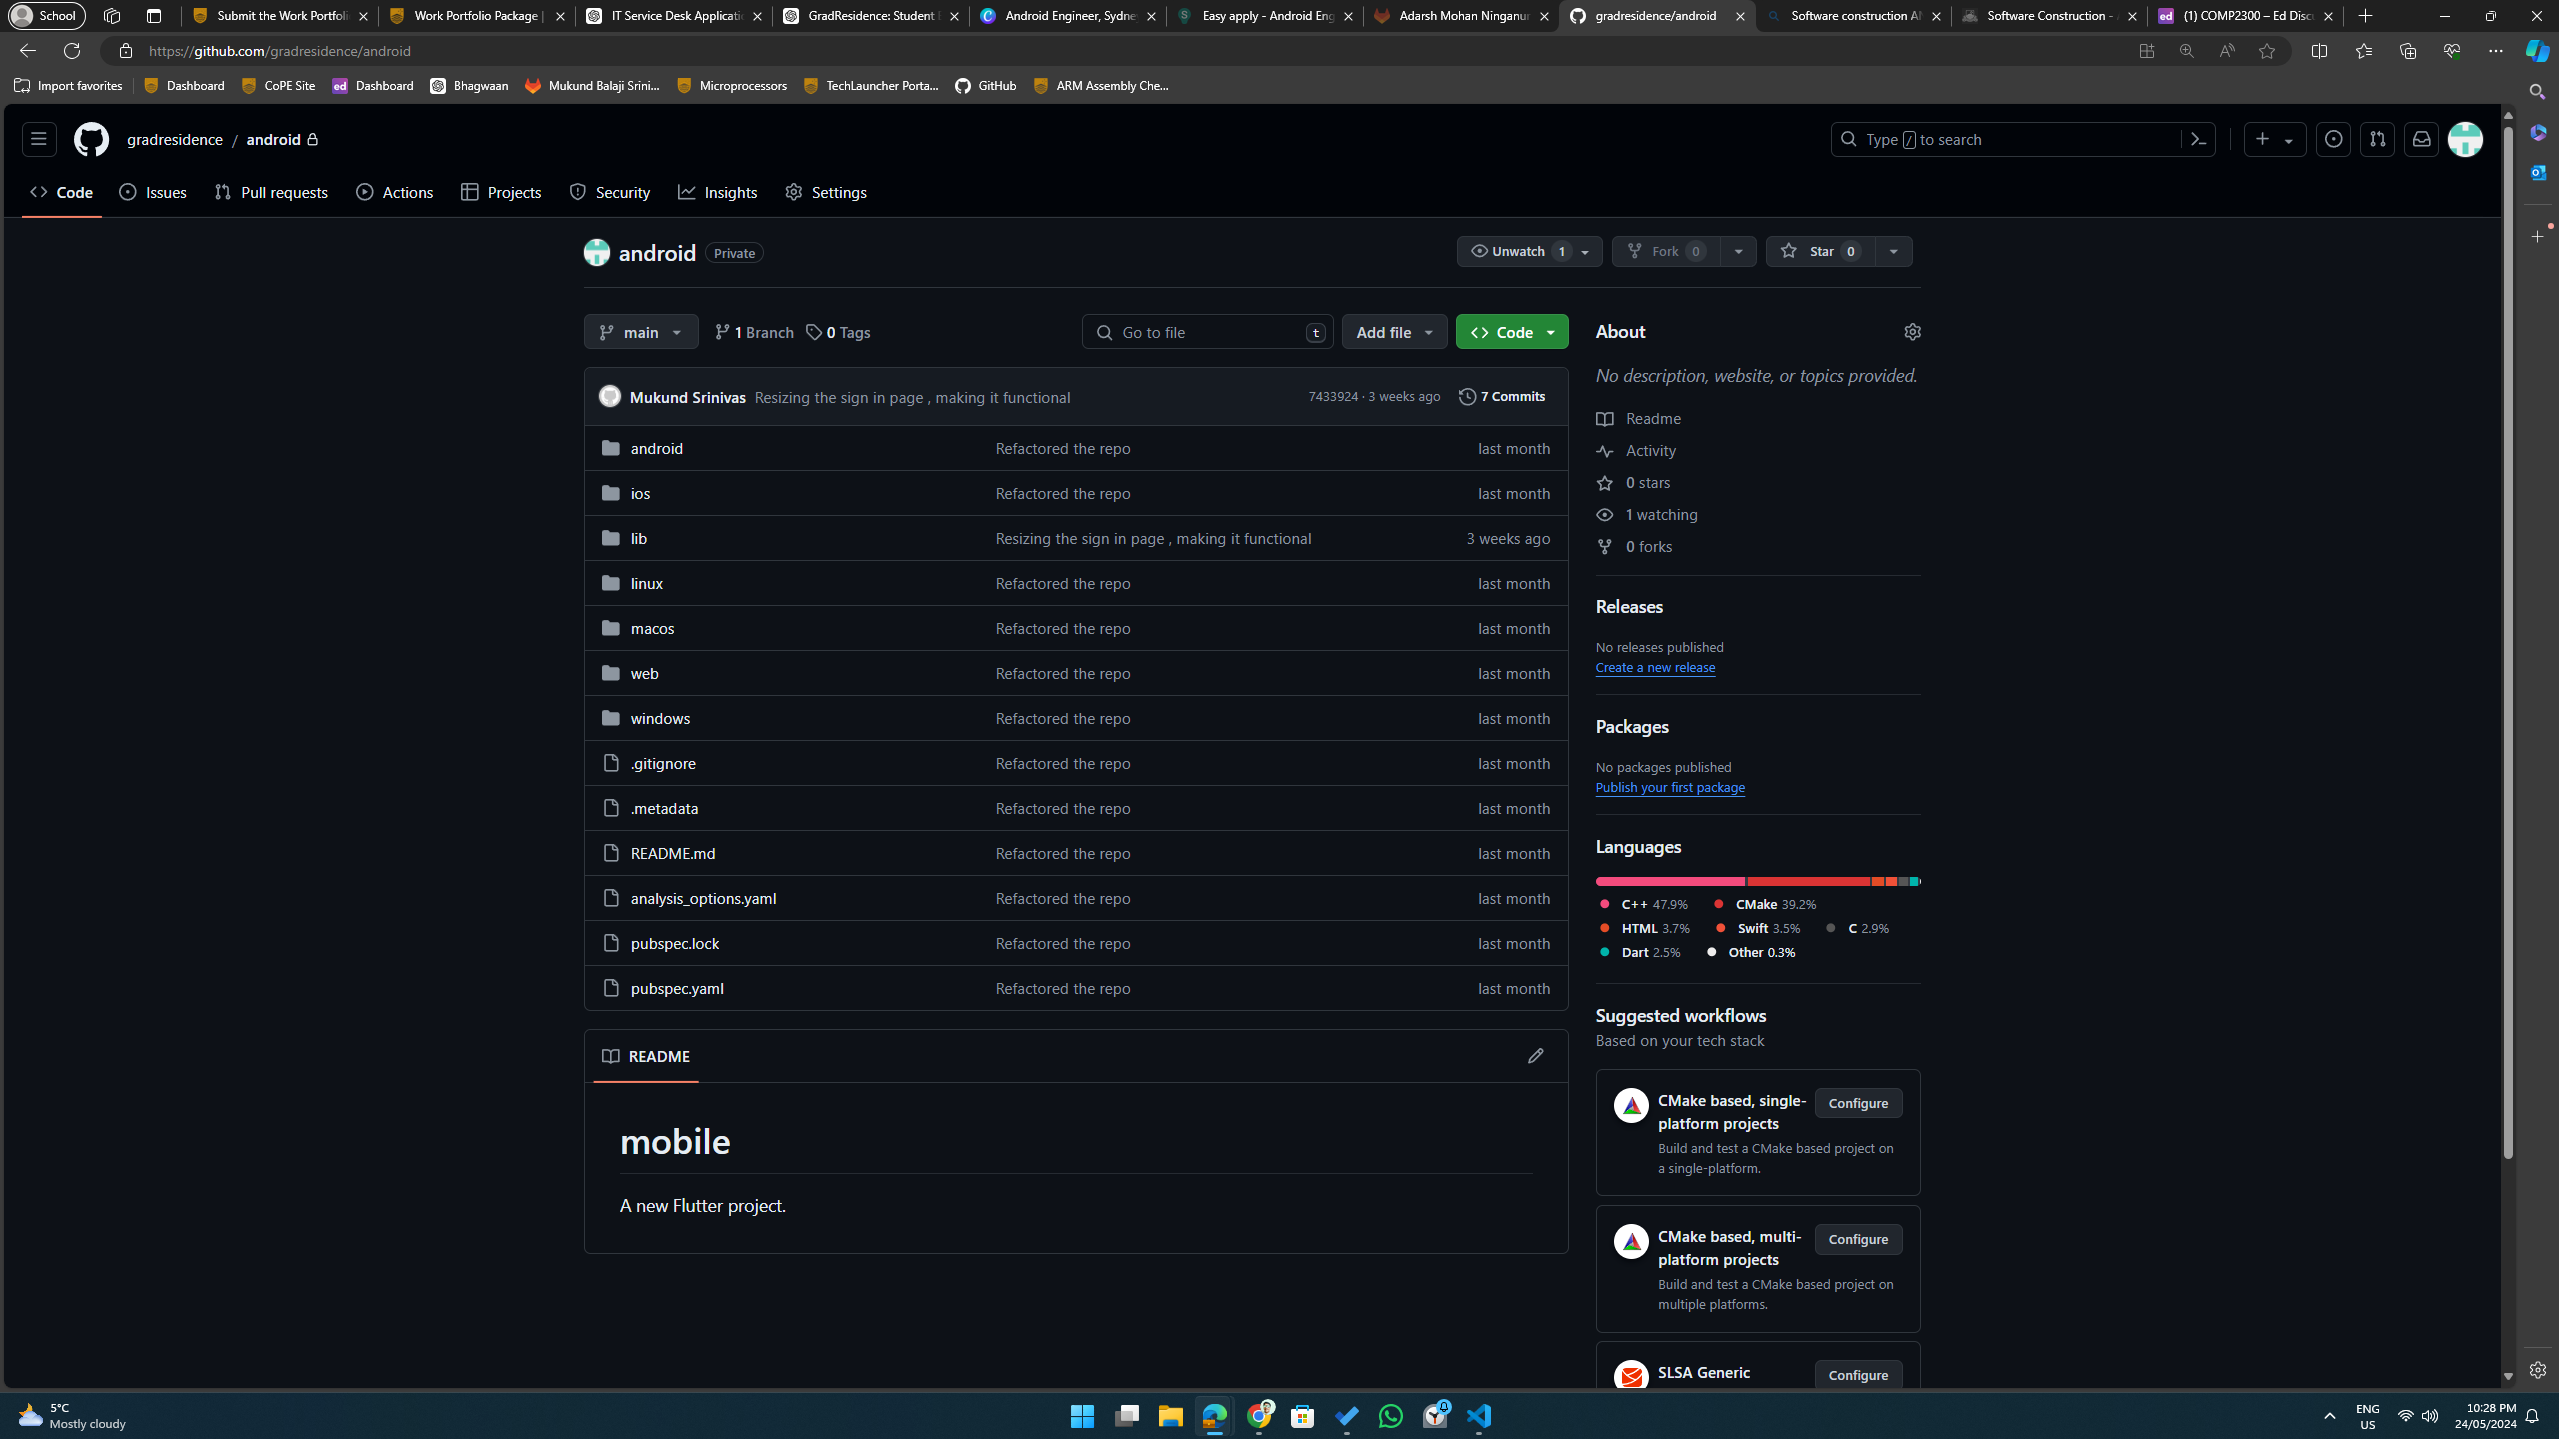
\includegraphics[width=\textwidth, height=0.4\textheight, keepaspectratio]{../gradResidence_Android.png}
    \caption{Screenshot of the GradResidence Android GitHub directory.}
    \label{fig:gradResidenceAndroid}
\end{figure}

\vspace{1cm}

\begin{figure}[ht!]
    \centering
    
\includegraphics[width=\textwidth, height=0.4\textheight, keepaspectratio]{../PMICanberra_Work.png}
    \caption{Screenshot of the Website Developed using MailChimp}
    \label{fig:PMI Canberra}
\end{figure}

\begin{figure}[ht!]
    \centering
    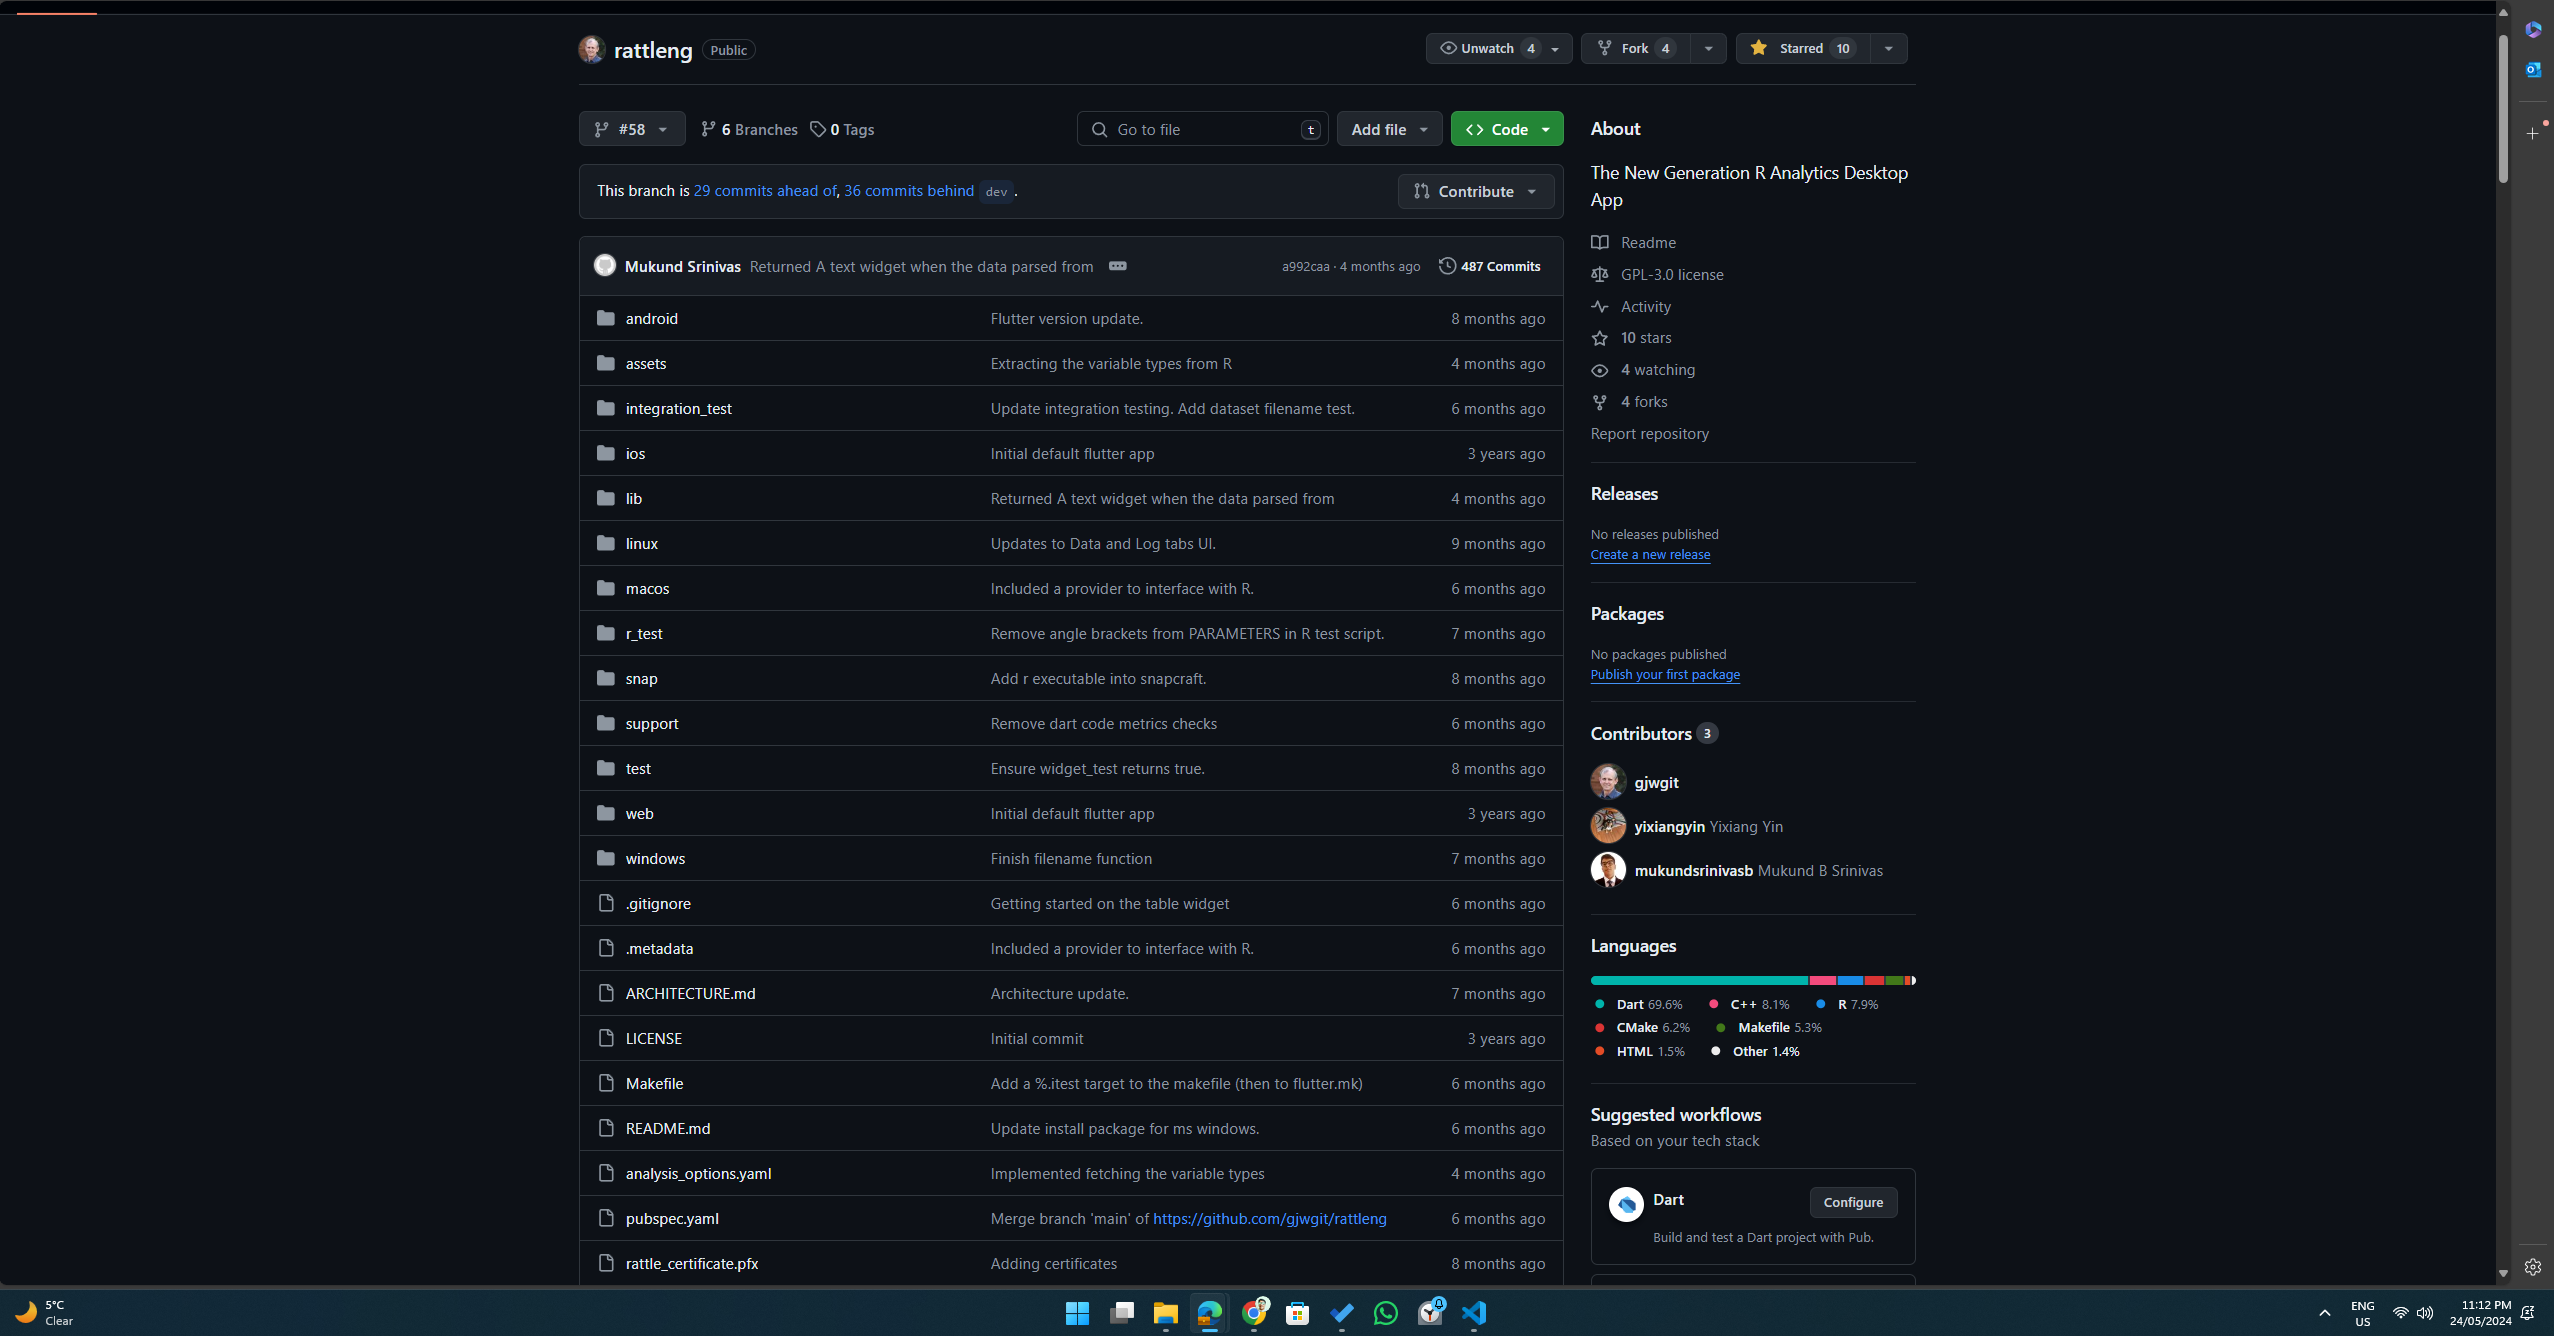
\includegraphics[width=\textwidth, height=0.4\textheight, keepaspectratio]{../rattleng_Experience.png}
    \caption{Proof of Contribution to the RattleNG project}
    \label{fig:RattleNG}
\end{figure}

\begin{figure}[ht!]
    \centering
    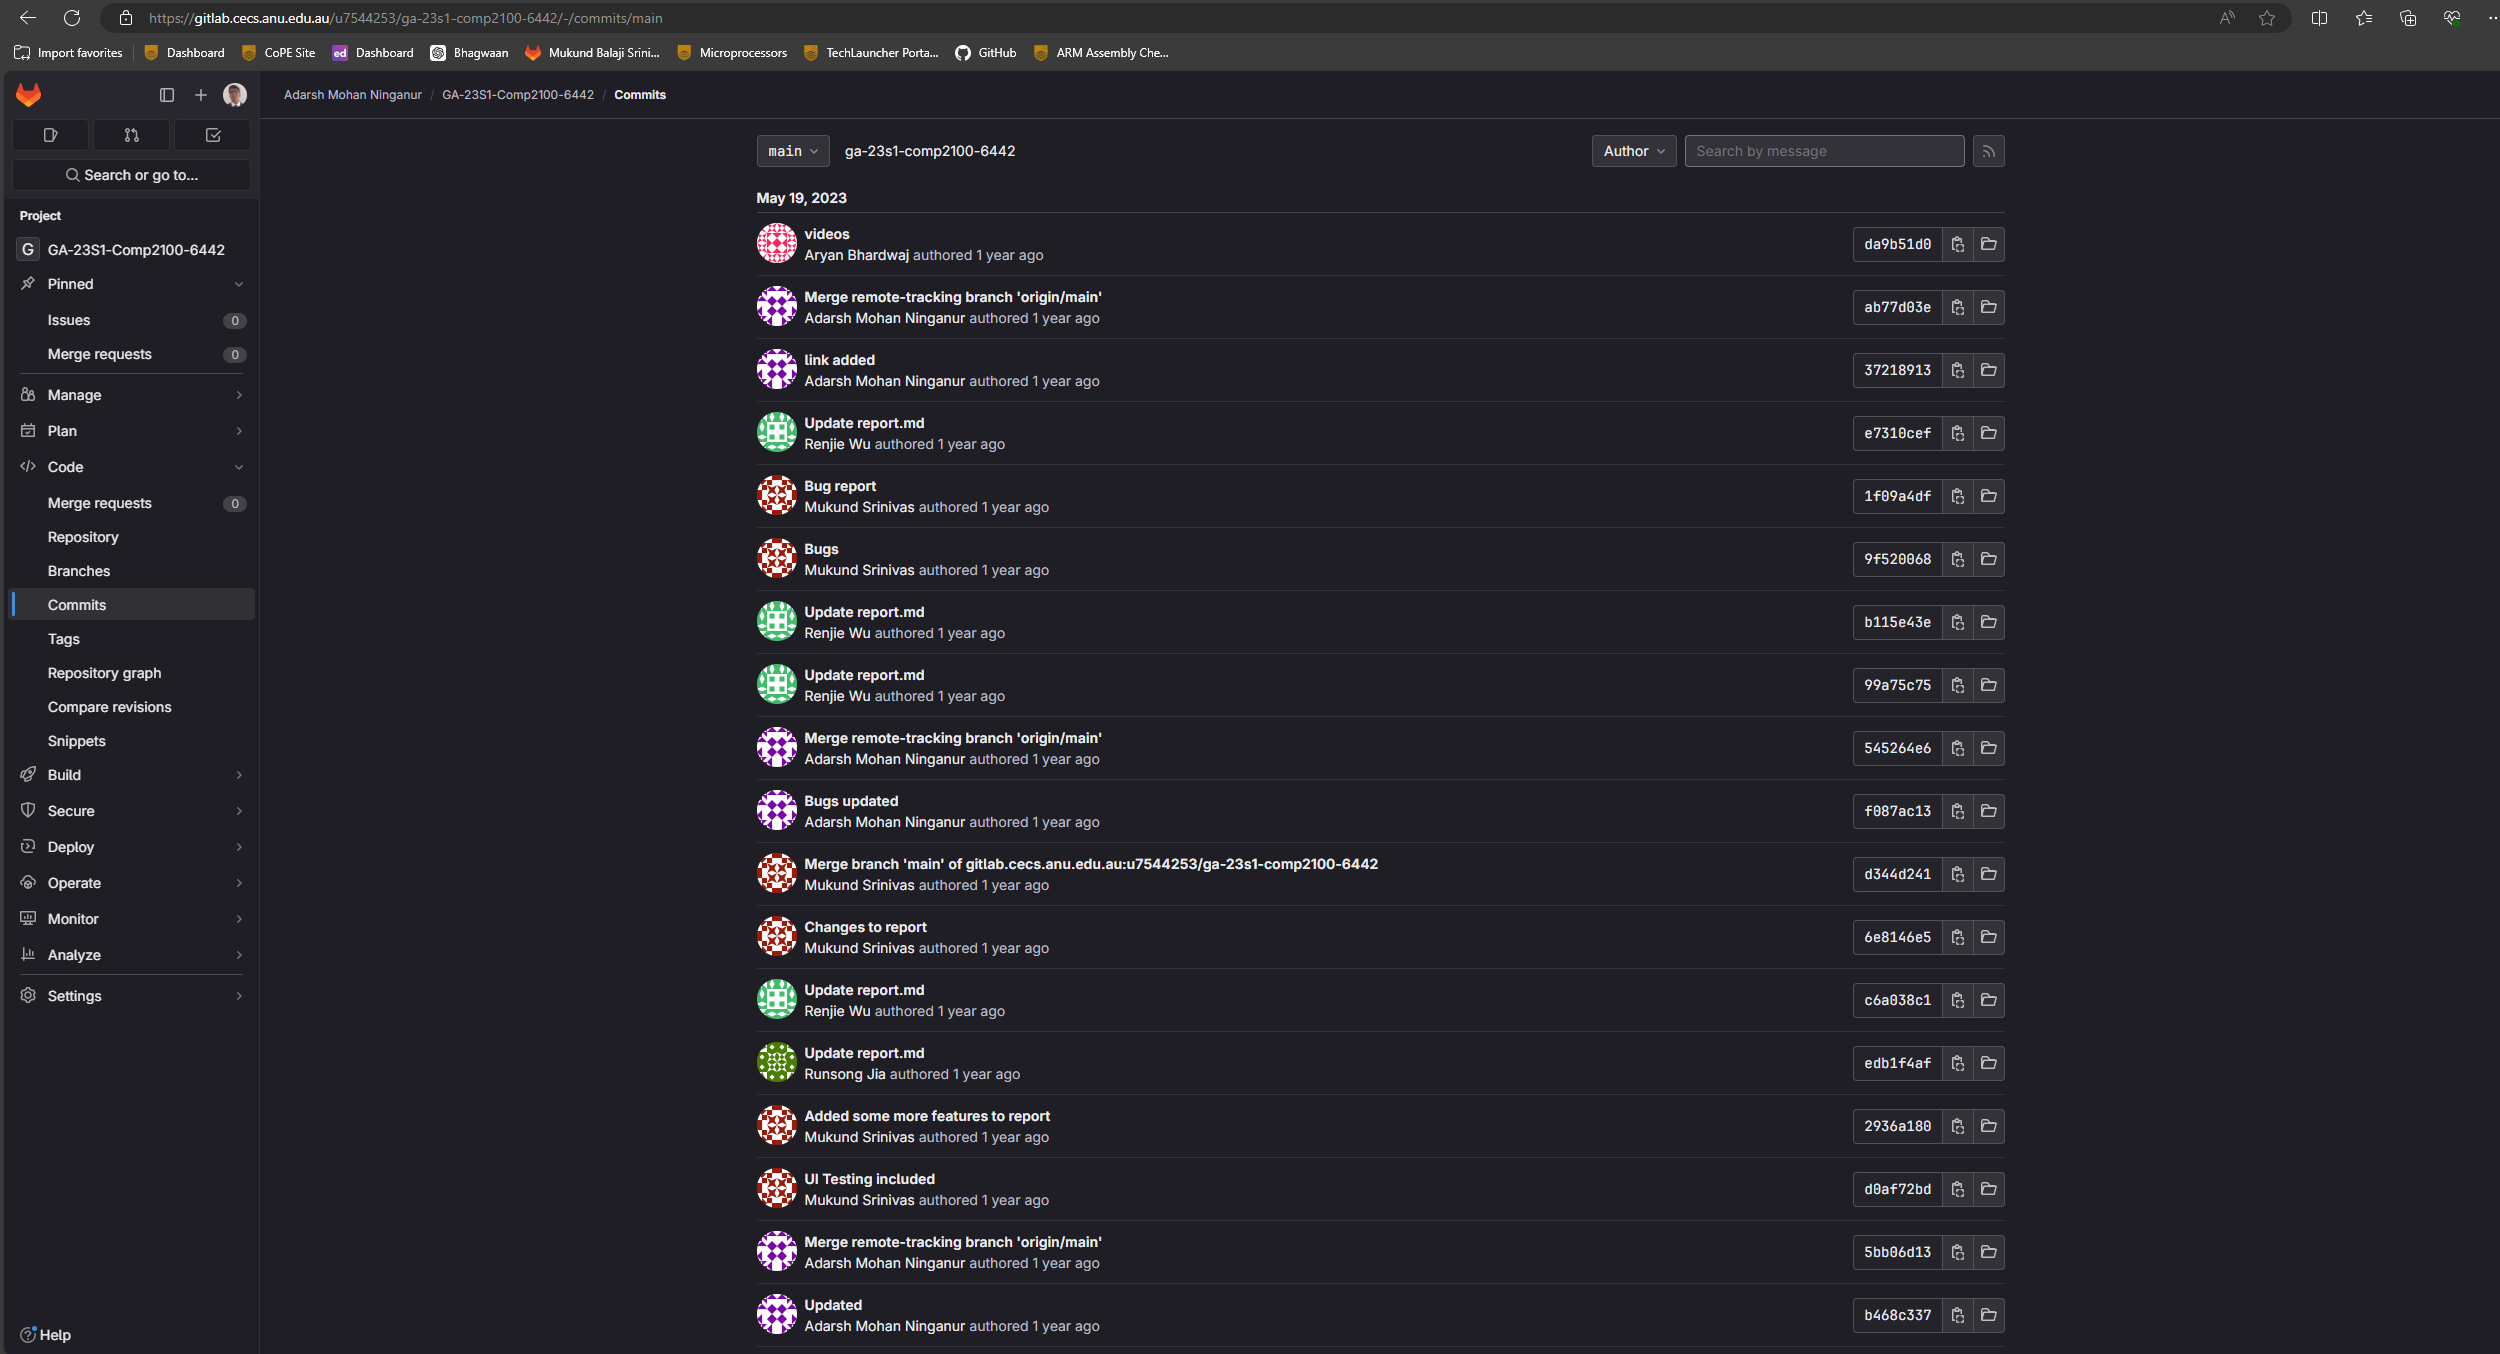
\includegraphics[width=\textwidth, height=0.4\textheight, keepaspectratio]{../Software_Construction_Proof.png}
    \caption{Proof of Contribution to Software Construction Project}
    \label{fig:Software Construction}
\end{figure}

\vspace{1cm}

\begin{figure}[h!]
    \centering
    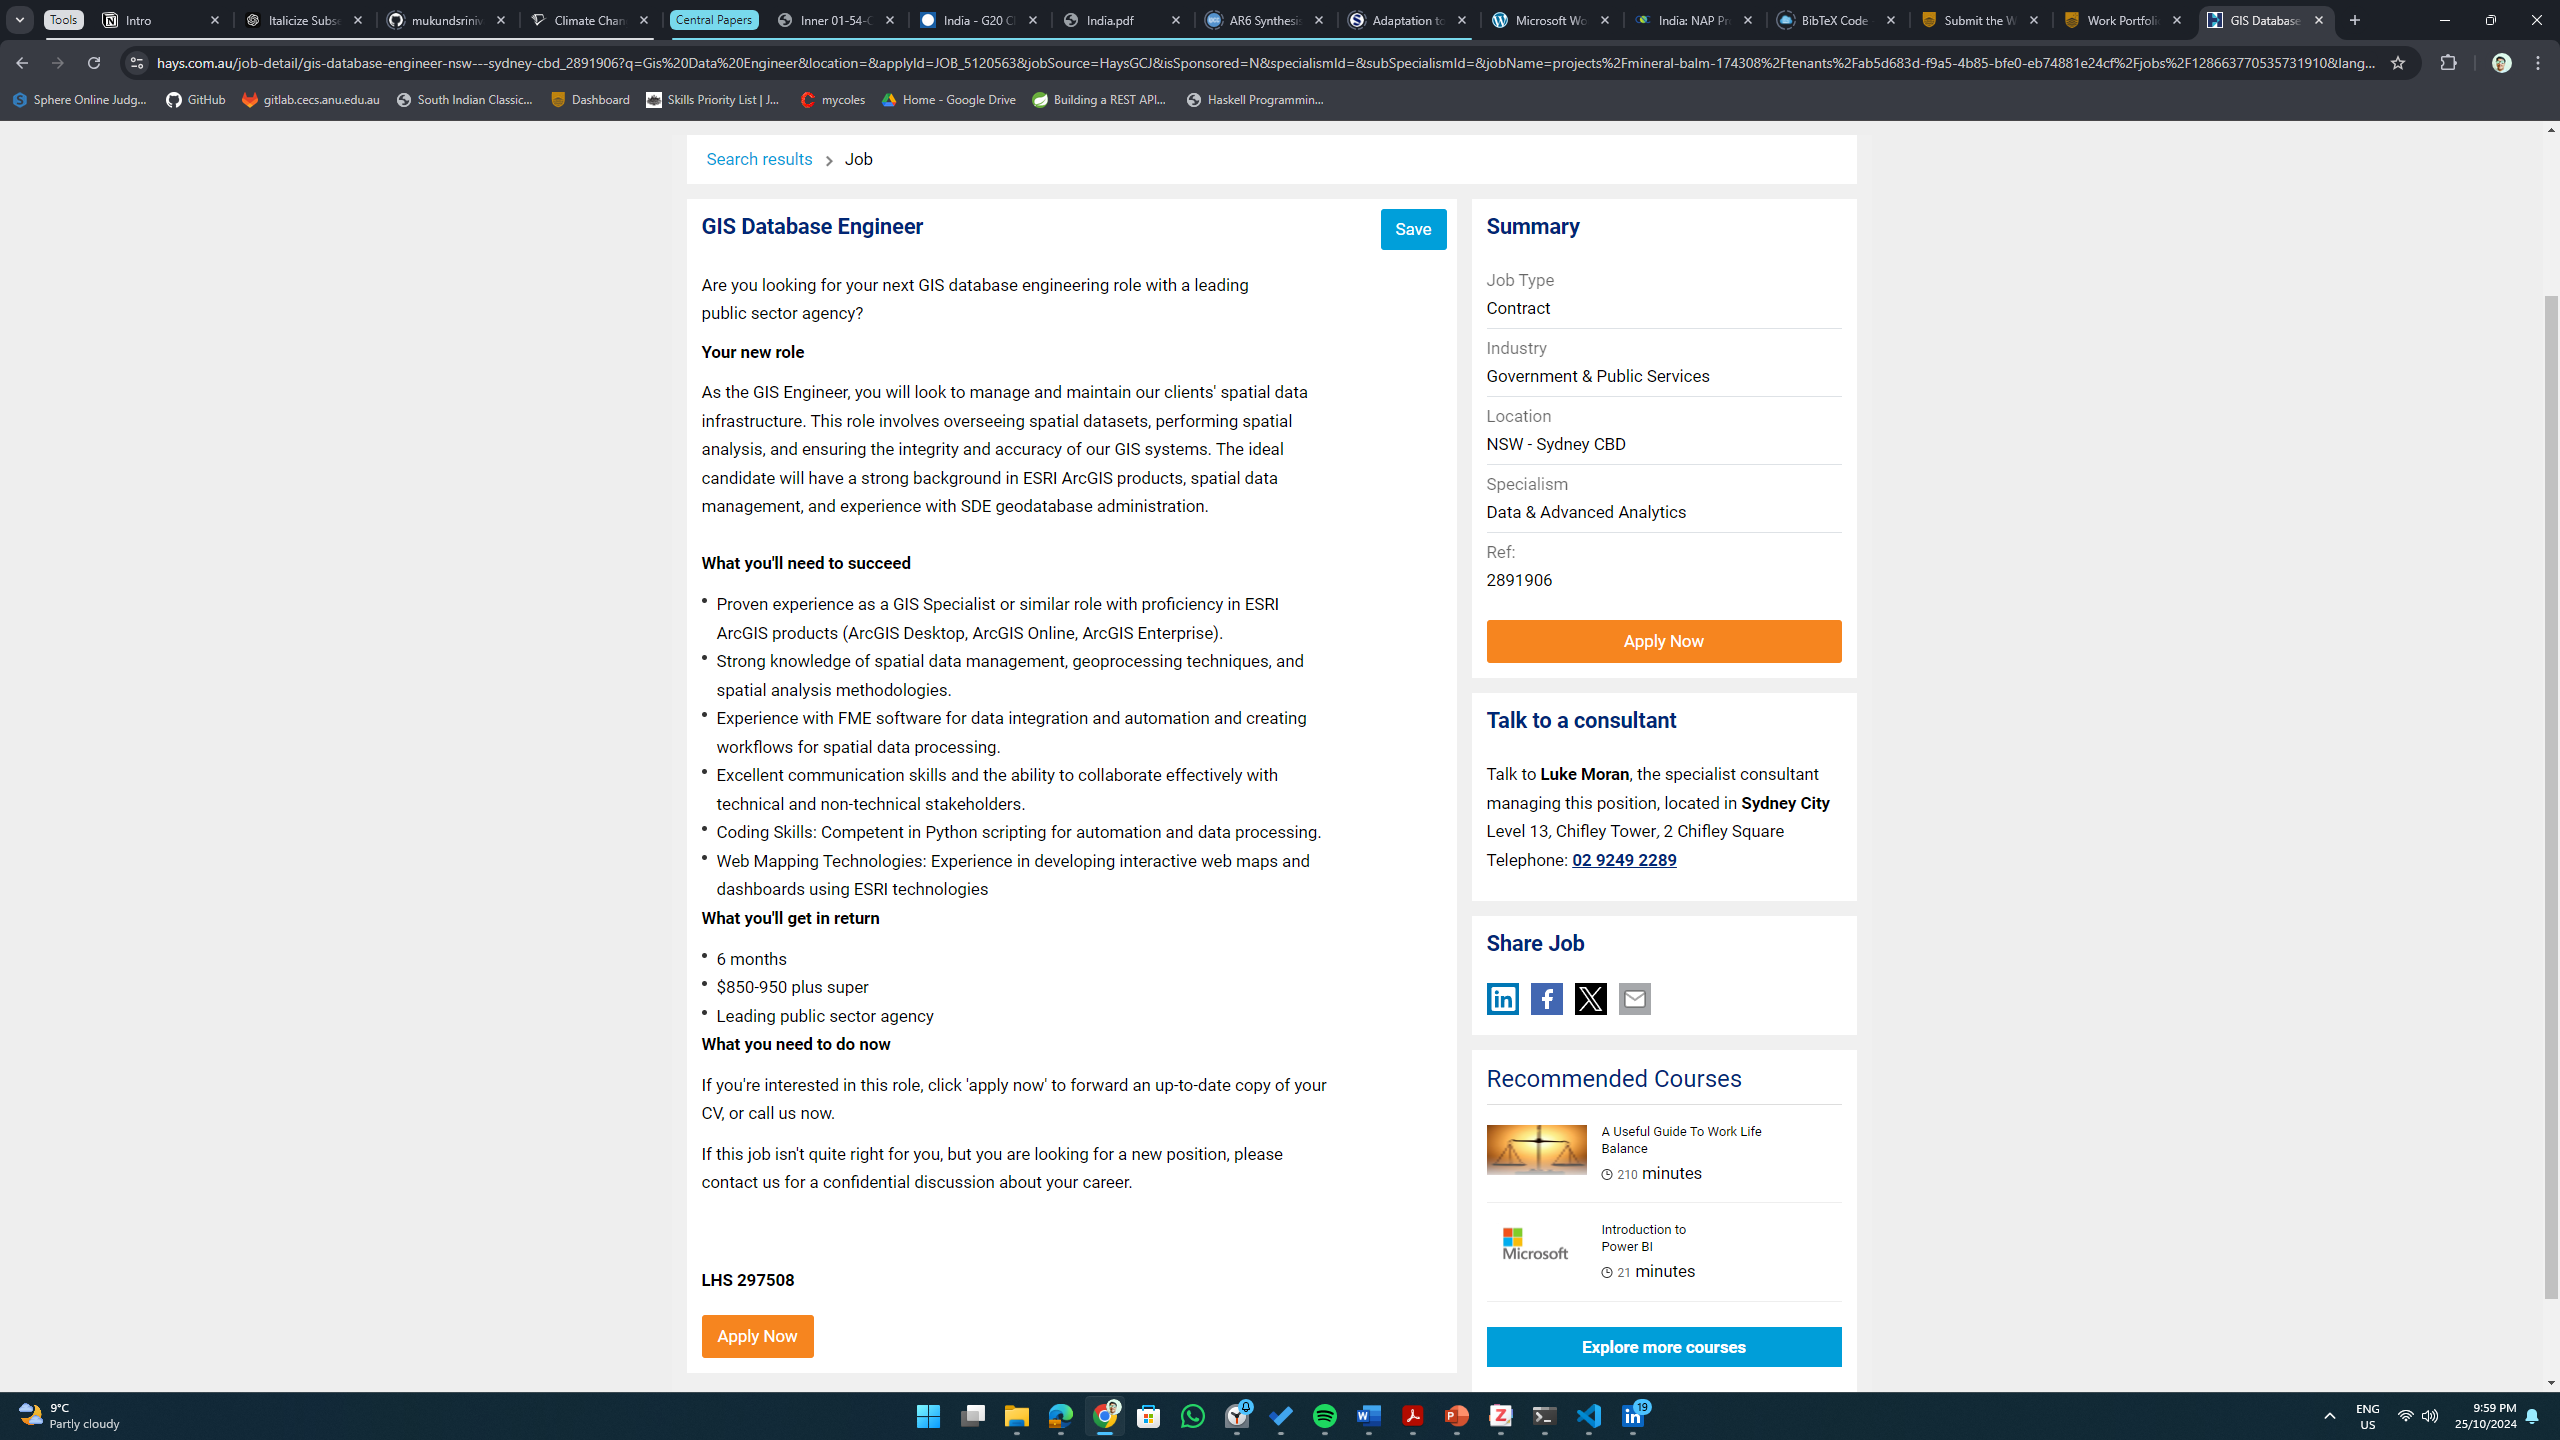
\includegraphics[width=\textwidth]{../job_posting_gis.png}
    \caption{Screenshot of the GIS Database Engineer job posting advertised by hays.}
    \label{fig:Job with hays}
\end{figure}

\begin{figure}[h!]
    \centering
    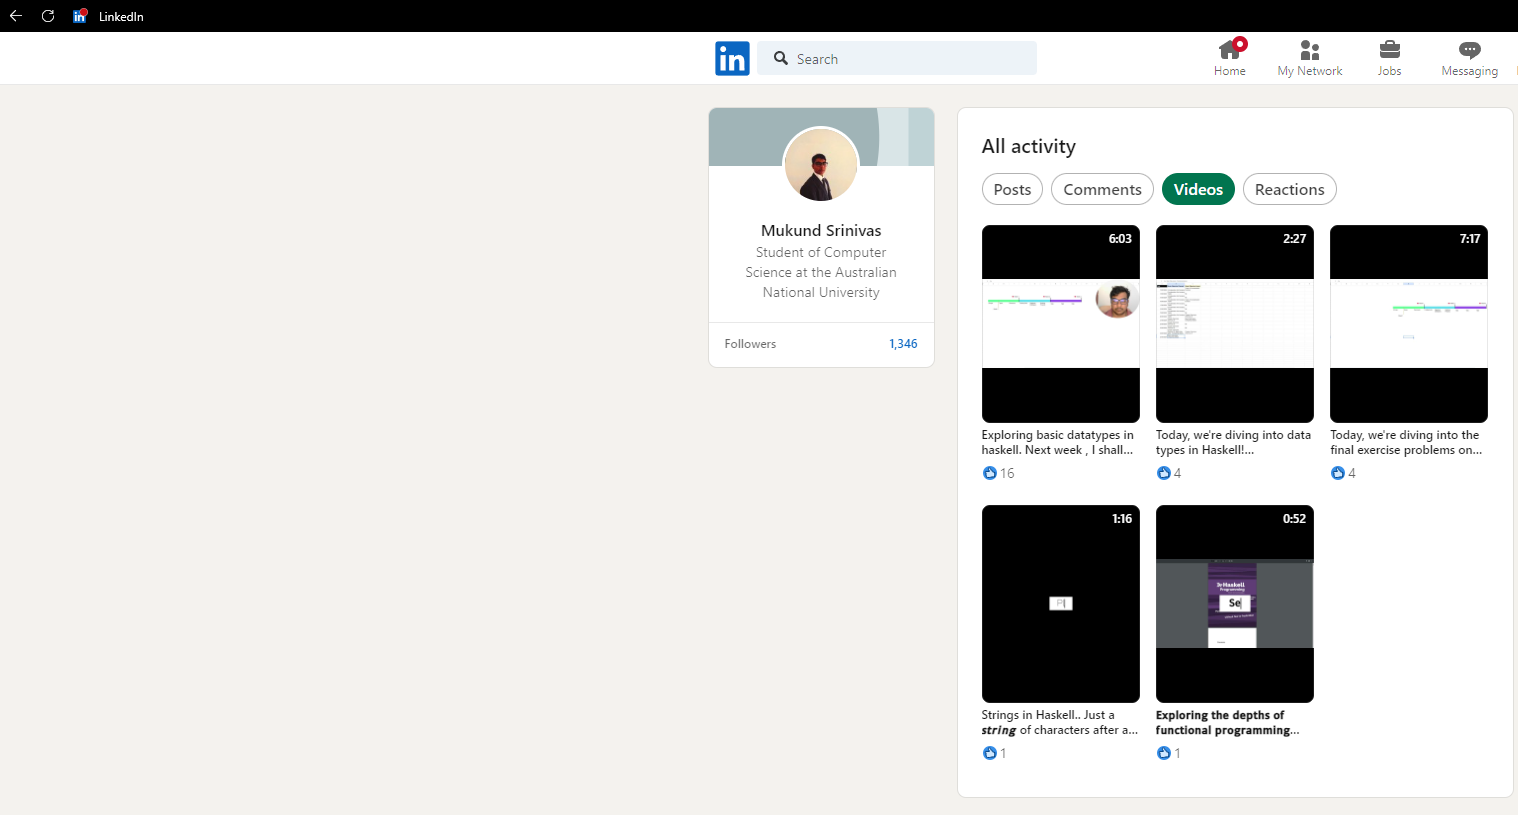
\includegraphics[width=\textwidth]{../haskell_videos_posting.png}
    \caption{Proof of Posting Educational Content.}
    \label{fig:Linkedin Content }
\end{figure}


\begin{figure}[h!]
    \centering
    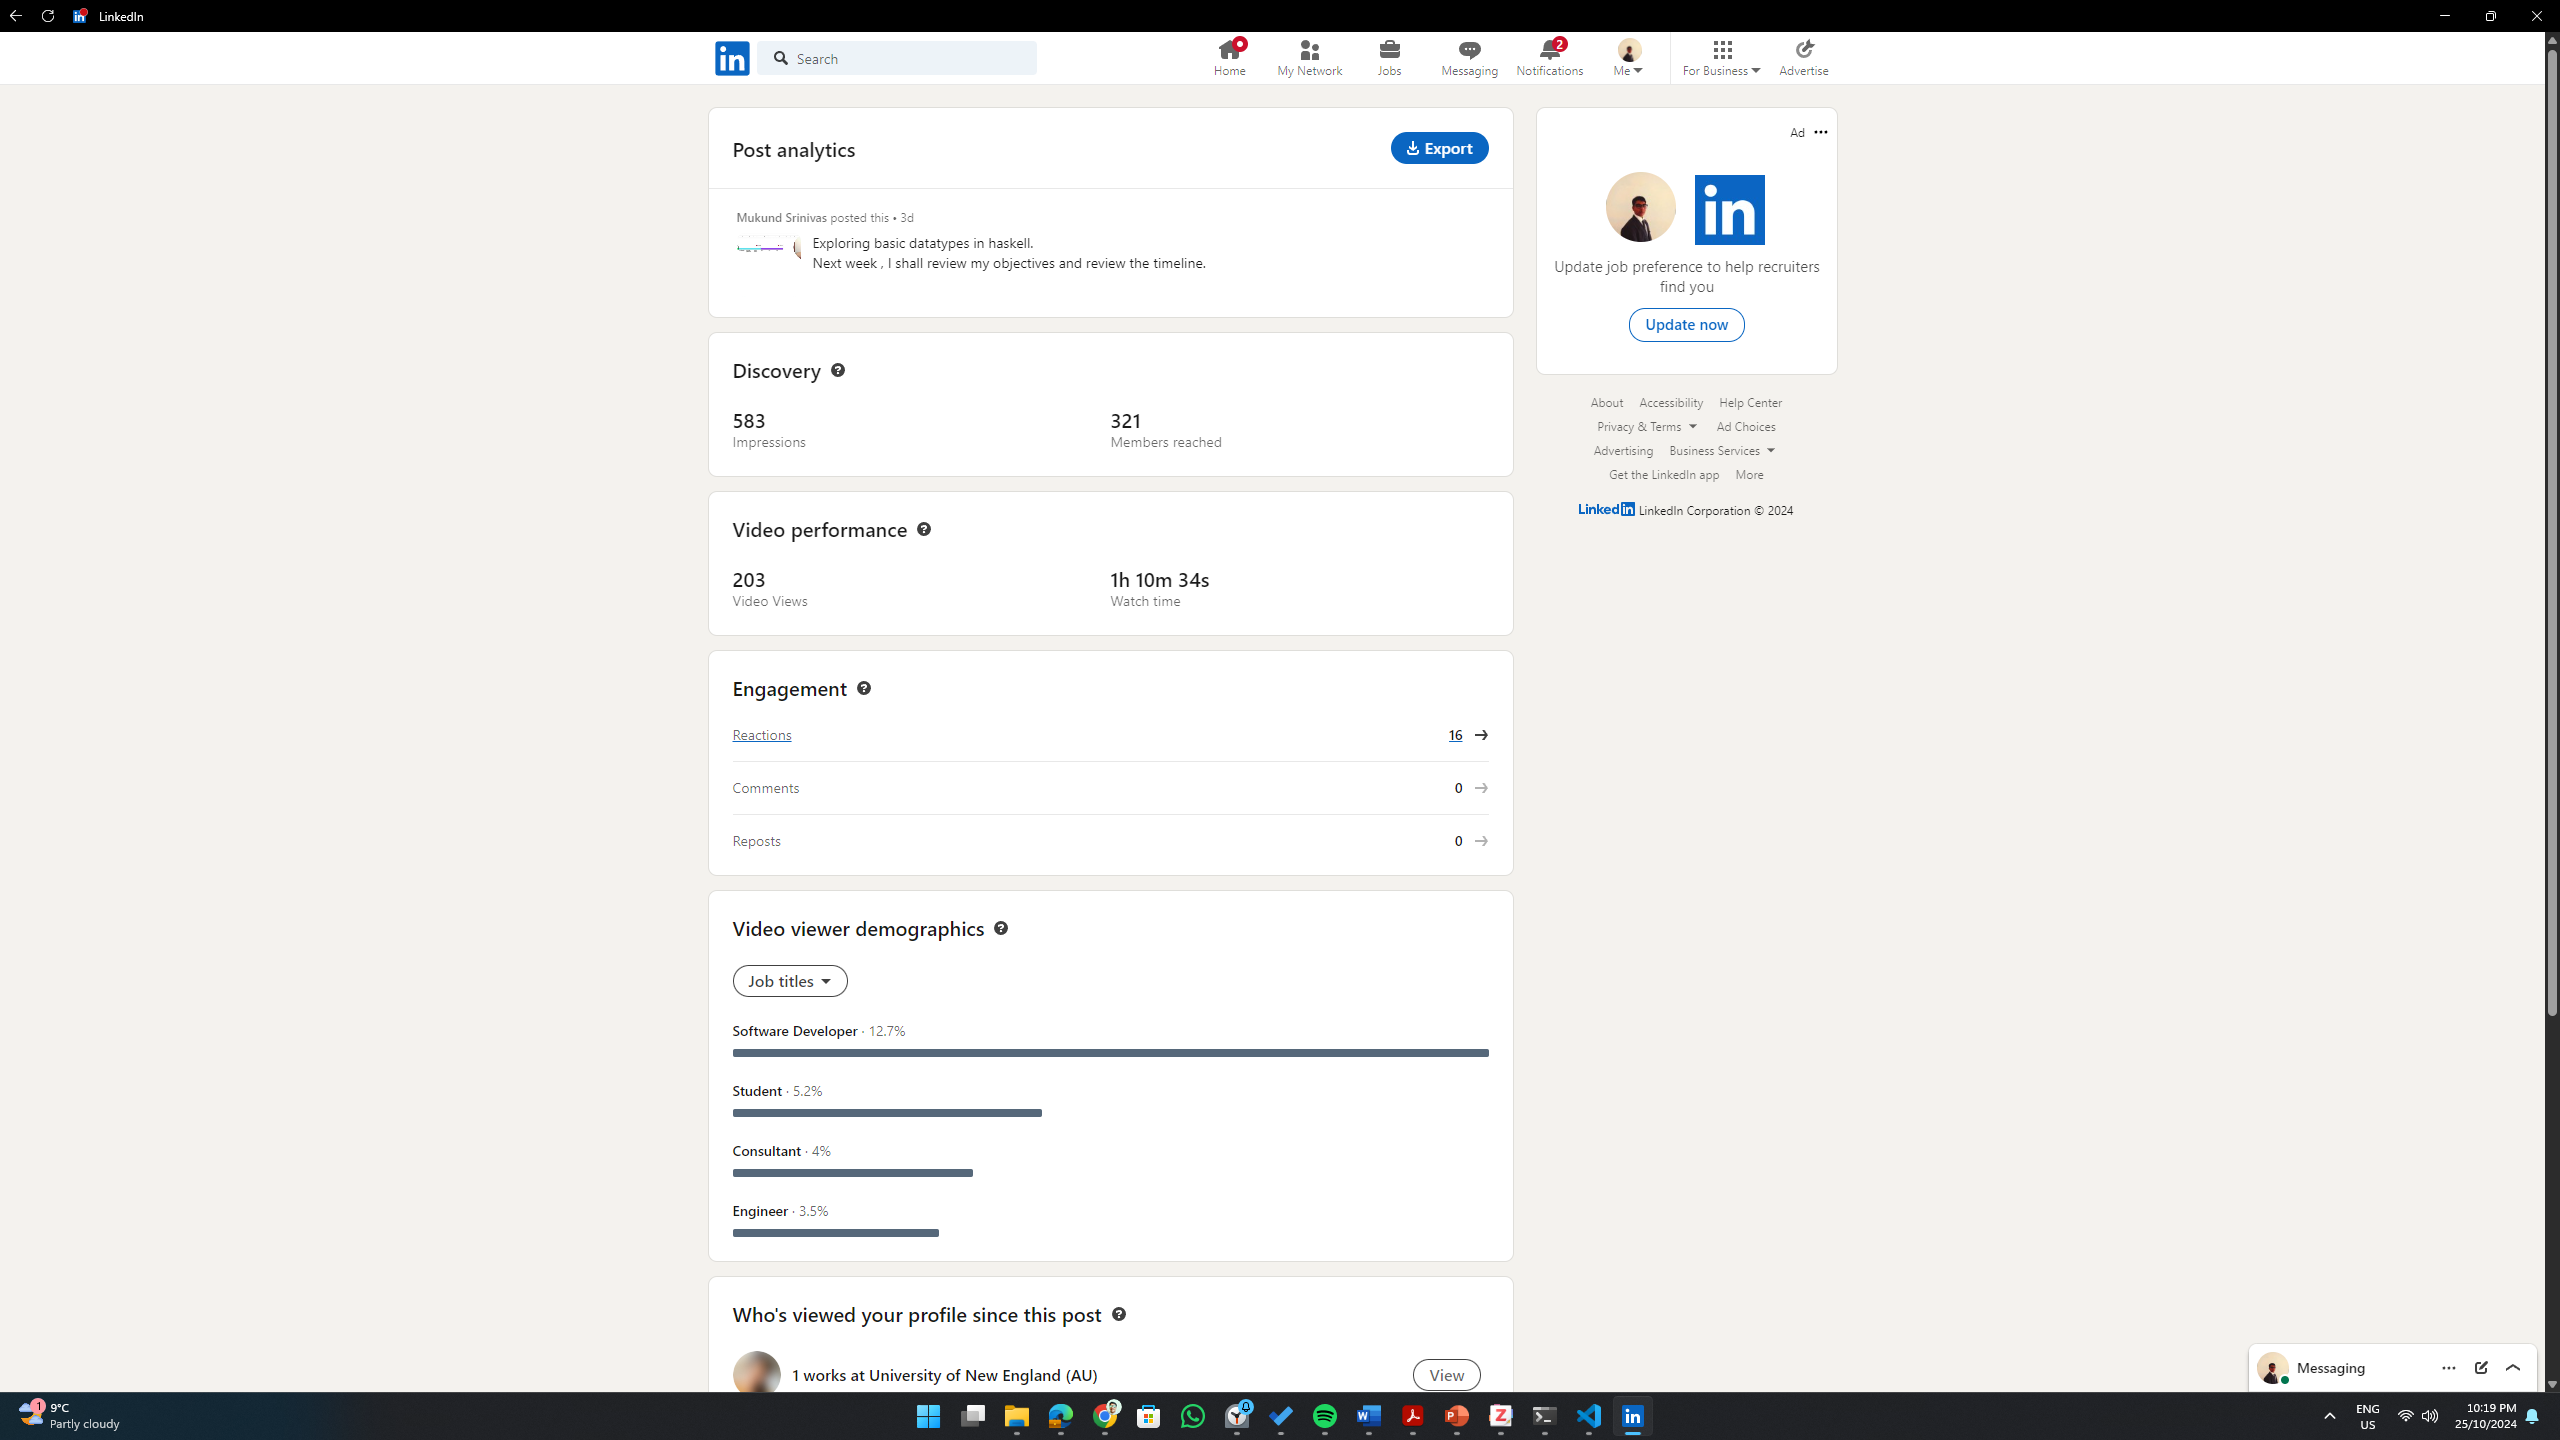
\includegraphics[width=\textwidth]{../Analytics_on_latest_video.png}
    \caption{Analytics on the latest video.}
    \label{fig:Linkedin Content-2}
\end{figure}



\end{document}
